%%%%%%%%%%%%%%%%%%%%%%%%%%%%%%%%%%%%%%%%%%%%%%%%%%%%%%%%%%%%%%%%%%%%%%%%%%%%%%%%
%%
%%   BornAgain Physics Manual
%%
%%   homepage:   http://www.bornagainproject.org
%%
%%   copyright:  Forschungszentrum Jülich GmbH 2015
%%
%%   license:    Creative Commons CC-BY-SA
%%
%%   authors:    Scientific Computing Group at MLZ Garching
%%               C. Durniak, M. Ganeva, G. Pospelov, W. Van Herck, J. Wuttke
%%
%%%%%%%%%%%%%%%%%%%%%%%%%%%%%%%%%%%%%%%%%%%%%%%%%%%%%%%%%%%%%%%%%%%%%%%%%%%%%%%%

% \part{Reference}\label{PREF}

\chapter{Simulation, Instrument, Histograms}\label{SRefBas}

%%%%%%%%%%%%%%%%%%%%%%%%%%%%%%%%%%%%%%%%%%%%%%%%%%%%%%%%%%%%%%%%%%%%%%%%%%%%%%%%
\section{Simulation classes}\label{SRefSim}
%%%%%%%%%%%%%%%%%%%%%%%%%%%%%%%%%%%%%%%%%%%%%%%%%%%%%%%%%%%%%%%%%%%%%%%%%%%%%%%%

Each BornAgain simulation is run from one of the three
foundational simulation classes:\footnote
{Developer note: They all inherit from a common non-public (pure virtual)
interface class \ttIdx{Simulation}.}
\ttIdx{GISAS\-Simulation},
\ttIdx{OffSpecularSimulation},
\ttIdx{SpecularSimulation}.

%===============================================================================
\subsection{GISAS\-Simulation}
%===============================================================================

Class \ttIdx{GISAS\-Simulation} controls one
grazing-incidence small-angle scattering simulation.
The following six functions from the C$++$ API are sufficient to set up and run a basic
simulation:
\setCpp
\begin{lstlisting}
class GISASSimulation {
  GISASSimulation(); // constructor
  void setDetectorParameters(...);
  void setBeamParameters(...);
  void setSample(...);
  void runSimulation();
  Histogram2D* getIntensityData(...);
};
\end{lstlisting}
\constrHide{GISAS\-Simulation}%
They shall now be explained with full signatures.
Some alternatives will also be shown.

%--------------------------------------------------------------------------------
\begin{figure}[tb]
\begin{center}
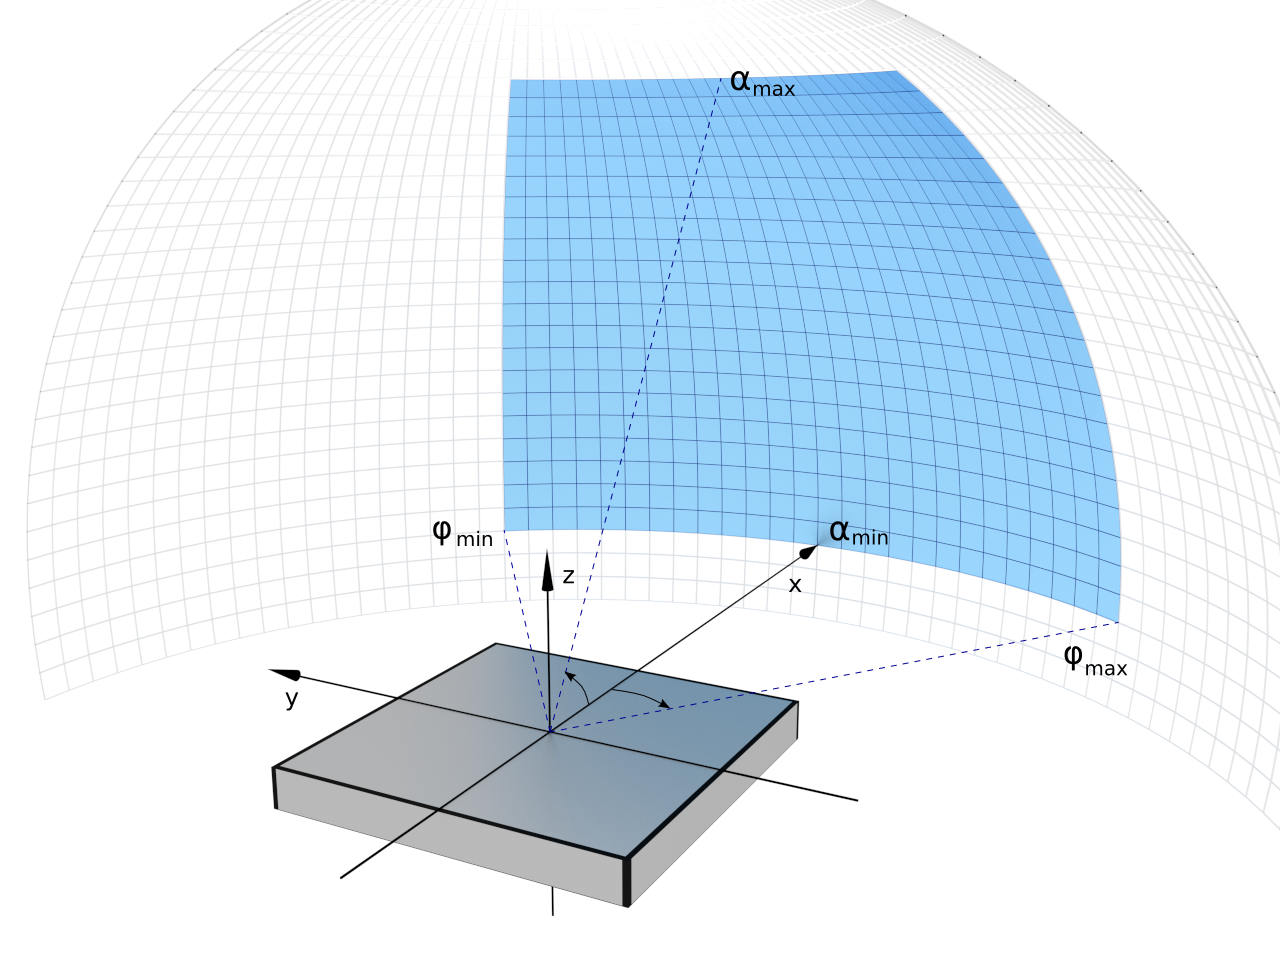
\includegraphics[width=0.7\textwidth]{fig/drawing/gisas_spherical_detector.png}
\end{center}
\caption{A spherical detector, with geometric conventions for polar angles~$\alpha$
and azimuthal angles~$\varphi$}
\label{FDetSpher}
\end{figure}
%--------------------------------------------------------------------------------

A two-dimensional detector must be defined through on of the following calls:

\subsubsection{Detector setup}\label{SRefDet}
\begin{lstlisting}
class GISASSimulation {
  void setDetectorParameters(
    size_t n_phi,   double phi_min,   double phi_max,
    size_t n_alpha, double alpha_min, double alpha_max);
  void setDetector(const IDetector2D& detector);
};
\end{lstlisting}
The function \clFct{GISAS\-Simulation}{setDetectorParameters}
defines a \ttIdx{SphericalDetector}
\index{Detector!spherical}%
with \texttt{n\_phi} equidistant azimuthal ($xy$, horizontal, off-specular) bins
\index{Azimuthal angle}%
\index{Horizontal angle}%
\index{Off-specular angle}%
\index{Angle!azimuthal ($=$ horizontal)}%
and  \texttt{n\_alpha} equidistant polar ($xz$, vertical, specular) bins (\cref{FDetSpher}).
\index{Polar angle}%
\index{Vertical angle}%
\index{Specular angle}%
\index{Angle!polar ($=$ vertical)}%

The alternate function~\clFct{GISAS\-Simulation}{setDetector}
allows to supply any detector that realizes the interface \ttIdx{IDetector2D}.
Besides \texttt{SphericalDetector}, this can be a \ttIdx{Rectangular\-Detector}.
For details, see the \tuto{141}{rectangular detector tutorial}.

\subsubsection{Beam setup}\label{SRefBeam}
\begin{lstlisting}
class GISASSimulation {
  void setBeamParameters(
    double wavelength, double alpha_i, double phi_i);
};
\end{lstlisting}
This function\clFctHide{GISAS\-Simulation}{setBeamParameters}
is rather self-explanatory.
The incident radiation wavelength must be given in the same length unit
that is also used in the sample description.

\subsubsection{Sample setup}
\begin{lstlisting}
class GISASSimulation {
  GISASSimulation(const MultiLayer& p_sample);
  GISASSimulation(const std::shared_ptr<IMultiLayerBuilder> p_sample_builder);
  void setSample(const MultiLayer& sample);
  void setSampleBuilder(const std::shared_ptr<IMultiLayerBuilder> p_sample_builder);
};
\end{lstlisting}
Besides function \clFct{GISAS\-Simulation}{setSample}, there is an alternate
function \clFct{GISAS\-Simulation}{setSampleBuilder}.
Either function call can be replaced by an extend forms of the constructor
\constr{GISAS\-Simulation}.

Since BornAgain is only concerned with multilayer samples,
the \E{sample} class
\index{Sample (class)|see{\Code{MultiLayer}}}%
is called \ttIdx{MultiLayer},
and each \E{sample builder} must realize the interface \ttIdx{IMulti\-Layer\-Builder}.
\index{Sample builder (interface)|see{\Code{IMultiLayerBuilder}}}%

A sample builder provides a more versatile way to define a sample.
Usage examples can be found in the test cases in \ttIdx{Core/StandardSamples}
and in the Python example \ttIdx{FitSpheresInHexLattice\_builder.py}.

\subsubsection{Execution}
\begin{lstlisting}
class GISASSimulation {
  void runSimulation();
};
\end{lstlisting}
\clFctHide{GISAS\-Simulation}{runSimulation}%
Once the simulation is fully set up, it is run once through this command.
Results are stored in a protected class variable.

\subsubsection{Retrieval of result}
\begin{lstlisting}
class GISASSimulation {
  Histogram2D* getIntensityData(AxesUnits units_type = AxesUnits::DEFAULT) const;
};
\end{lstlisting}
\clFctHide{GISAS\-Simulation}{getIntensityData}%
This function returns a pointer to a \ttIdx{Histogram2D}
that contains the outcome of the simulation.
% TODO link -> as further discussed in~\Cref{SRefHis2D}.

%===============================================================================
\subsection{Off\-Specular\-Simulation}
%===============================================================================

\MissingSection

%===============================================================================
\subsection{Specular\-Simulation}
%===============================================================================

\MissingSection

%%%%%%%%%%%%%%%%%%%%%%%%%%%%%%%%%%%%%%%%%%%%%%%%%%%%%%%%%%%%%%%%%%%%%%%%%%%%%%%%
\section{Intensity data}
%%%%%%%%%%%%%%%%%%%%%%%%%%%%%%%%%%%%%%%%%%%%%%%%%%%%%%%%%%%%%%%%%%%%%%%%%%%%%%%%

\MissingSection
\iffalse

%===============================================================================
\subsection{Histogram2D}\label{SRefHis2D}
%===============================================================================

\Work{The following material has been moved here from a Tutorial.
It still needs to be recast in Reference style.}

The \Code{IntensityData} object stores the
simulated or real intensity data together with the axes definition of the detector in BornAgain's internal format.
During the simulation setup
it is created automatically when the user specifies the detector characteristics and is filled with the simulated intensities after the simulation is completed.

\setPy
\begin{lstlisting}
simulation = Simulation()
simulation.setDetectorParameters(10, -5.0*degree, 5.0*degree, 5, 0.0*degree, 1.0*degree)
...
simulation.runSimulation()
intensity = simulation.getIntensityData() @\label{py:UserApi:intensity}@
\end{lstlisting}

The \Code{IntensityData} object retrieved in line~\ref{py:UserApi:intensity} corresponds to
the two dimensional detector pixel array as shown in \cref{fig:UserApi:IntensityData}.

\begin{figure}[ht]
  \centering
    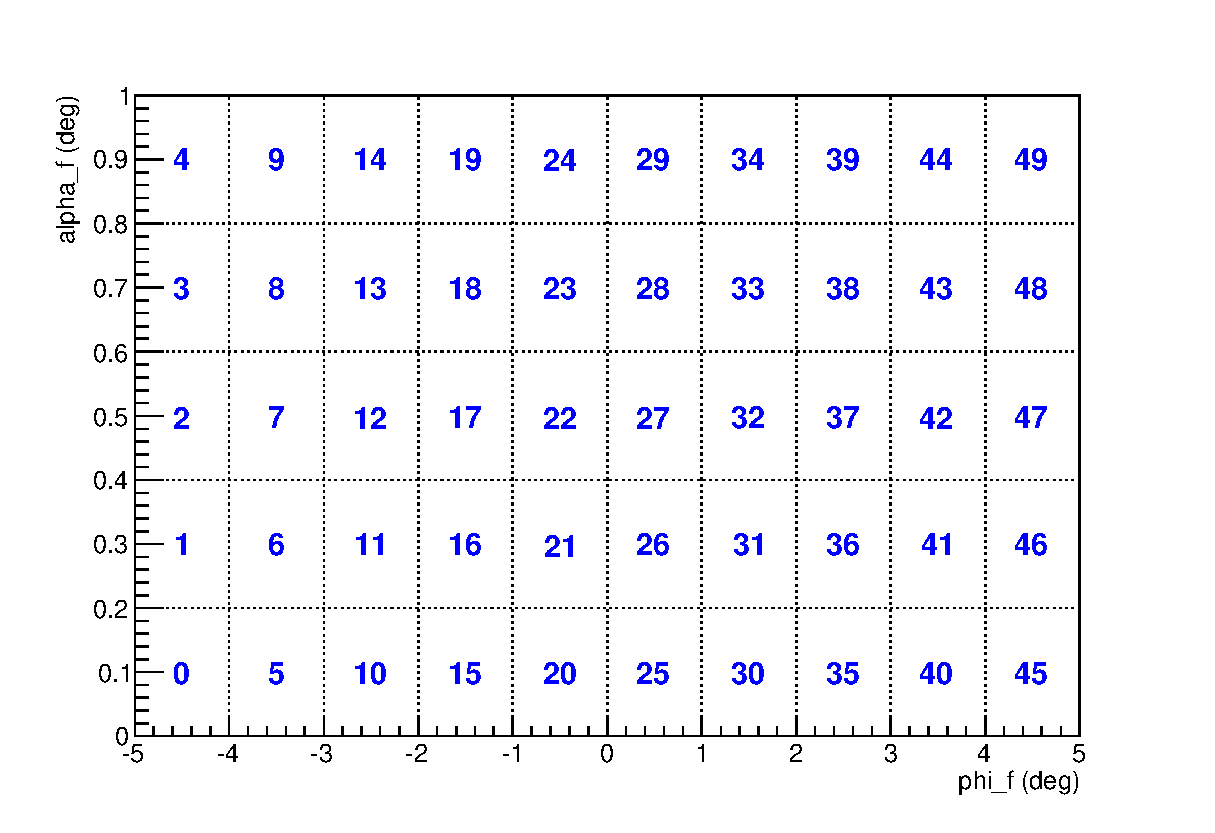
\includegraphics[clip=, width=120mm]{fig/drawing/UserAPI_IntensityDataLayout.eps}
  \caption{The axes layout of IntensityData object.}
  \label{fig:UserApi:IntensityData}
\end{figure}

The x-axis and y-axis of the figure correspond to the $\phi_f$ and $\alpha_f$ axes of the detector.
The x-axis is divided into 10 bins,
with low edge of the first bin set to $-5.0\,{\rm deg}$ and upper edge of the last bin set to $+5.0\,{\rm deg}$.
The y-axis is divided into 5 bins,
with low edge of the first bin set to $0.0\,{\rm deg}$ and upper edge of the last bin set to $1.0\,{\rm deg}$.
There are 50 bins in total (they are marked on the plot with indexes from 0 to 49), each bin will contain one intensity value.

During a standard simulation (i.e. no Monte-Carlo integration involved) intensities are calculated for $\phi_f, \alpha_f$ values corresponding to the bin centers, e.g. the intensity stored in bin\#42 will correspond to $\phi_f=3.5\,{\rm deg}, \alpha_f=0.5\,{\rm deg}$.
\vspace*{2mm}


\Note{
The \Code{IntensityData} object is not intended for direct usage from Python API. The idea is
that the API provides the user with the possibility to export the data from BornAgain internal format to the format of his choice as well as import user's data into BornAgain.
For the moment this functionality is limited to a few options explained below.
We encourage users feedback to implement the support of most requested formats.}


\subsubsection{Import/export of intensity data}
For the moment we provide following options:
\begin{itemize}
\item Import/export of \Code{IntensityData} object from/to \Code{numpy} array.
\item Import/export of \Code{IntensityData} object from/to text file.

\end{itemize}

\paragraph{Export to numpy array}

To export intensity data into  \Code{numpy} array the method \Code{getArray()} should be used
on \Code{IntensityData} object as shown in line \ref{py:UserApi:getArray} of
following code snippet.

\begin{lstlisting}
intensity = simulation.getIntensityData()
array = intensity.getArray() @\label{py:UserApi:getArray}@
...
pylab.imshow(numpy.rot90(array, 1)) @\label{py:UserApi:imshow}@
pylab.show()
\end{lstlisting}

For the detector settings defined in the previous paragraph the dimensions of the resulting array will be (10,5). By using \Code{numpy} indexes the user can get access to the intensity values, e.g.
\Code{array[0][0]} corresponds to the intensity in bin\#0 of \cref{fig:UserApi:IntensityData},
\Code{array[0][4]} to bin\#4,
\Code{array[1][0]} to bin\#5,
\Code{array[8][2]} to bin\#42,
\Code{array[9][4]} to bin\#49.


To plot this resulting numpy array with \Code{matplotlib} it has to be rotated counter-clockwise
to match \Code{matplotlib} conventions as shown in line~\ref{py:UserApi:imshow}.


%\subsubsection{Direct access to the data}
%User can access to the

%\begin{lstlisting}[language=python, style=eclipseboxed]
%for i in range(0, intensity.getAllocatedSize()):
%    print intensity[i]
%\end{lstlisting}


\subsubsection{Importing from numpy array}

To use fitting the user has to load experimental data into BornAgain fitting kernel.
To read experimental data the user has to create
IntensityData object, fill it with the experimental  intensity values and pass
this object to the fitting kernel.

First, the user creates empty \Code{IntensityData} as shown
in line~\ref{py:UserApi:IntensityData} of the following code snippet.
\begin{lstlisting}
data = IntensityData() @\label{py:UserApi:IntensityData}@
data.addAxis(FixedBinAxis("phi_f", 10, -5.0*degree, 5.0*degree)) @\label{py:UserApi:phi_f}@
data.addAxis(FixedBinAxis("alpha_f", 5, 0.0*degree, 1.0*degree)) @\label{py:UserApi:alpha_f}@
...
array = numpy.zeros((10, 5)) # fill array with experimental intensities @\label{py:UserApi:create_array}@
...
data.setRawDataVector(array.flatten().tolist()) @\label{py:UserApi:set_raw}@

fitSuite = FitSuite() @\label{py:UserApi:fit_suite}@
fitSuite.addSimulationAndRealData(simulation, data) @\label{py:UserApi:add_real_data}@
\end{lstlisting}

In lines~\ref{py:UserApi:phi_f}, \ref{py:UserApi:alpha_f} two axes with fixed bin sizes
are defined to represent the detector layout as shown in \cref{fig:UserApi:IntensityData}.
The constructor of \Code{FixedBinAxis} object has the following signature

\begin{lstlisting}
FixedBinAxis(title, nbins, min_angle, max_angle)
\end{lstlisting}

The created \Code{IntensityData} object has to be filled with experimental intensities
using \Code{numpy} array prepared by the user (lines ~\ref{py:UserApi:create_array}-~\ref{py:UserApi:set_raw}). In lines \ref{py:UserApi:fit_suite},\ref{py:UserApi:add_real_data} the fitting kernel is created and initialized with \Code{Simulation} object and
\Code{IntensityData} object representing the experimental data.


\subsubsection{Saving intensity data to text file.}

The special class \Code{IntensityDataIOFactory} is intended for saving the intensity data
in different datafile formats. For the moment, it only supports saving the data in specific BornAgain's text files (the file extention \Code{*.int}).

\begin{lstlisting}
intensity = simulation.getIntensityData()
IntensityDataIOFactory.writeIntensityData(intensity, 'file_name.int')
\end{lstlisting}

\subsubsection{Reading intensity data from a text file.}
The same class is also intended for reading intensity data
from files with different formats. For the moment, it only supports reading the data from text files of special BornAgain's format (the file extention \Code{*.int}).

\begin{lstlisting}
intensity = IntensityDataIOFactory.readIntensityData('file_name.int')
\end{lstlisting}
\fi
